\section{Appendix A: Online Survey}

\noindent Survey Title: Working in Berlin without (fluent) German language skills

\subsection{Privacy Protection Notice / Datenschutzhinweis}

A complete privacy protection notice was included in English and German. The notice outlined that the survey “is part of a university research project on language requirements in Berlin’s job market. Participation is voluntary, and all responses will be anonymous and treated confidentially, in accordance with the EU General Data Protection Regulation (GDPR).” Respondents were also informed that we will collect “demographic information (e.g. age, education level, field of study) and your experiences with job searching in Berlin,” and that the results will be used “for academic purposes only and will not be shared with third parties. No personally identifying information (such as names, emails, or IP addresses) will be collected or stored.” Respondents were informed of their right to withdraw their participation at any time and that proceeding with the survey confirmed they were at least 18 years old and give informed consent for the use of their responses in this academic study.

\subsection{Questionnaire}
\begin{enumerate}
	\item Privacy Protection Notice acceptance (Required)
	\begin{description}
		\item[Note:] Those who disagreed with the notice were unable to continue with the rest of the survey's questions
	\end{description}
	\item Gender (Required)
	\begin{enumerate}
		\item Man
		\item Woman
		\item Non-binary
		\item Prefer not to say
	\end{enumerate}
	\item Age (Required)
	\begin{enumerate}
		\item < 18
		\item 18-25
		\item 26 – 35
		\item 36 – 45 
		\item > 55
		\item 	Prefer not to say
	\end{enumerate}
	\item Living district (Required)
	\begin{enumerate}
		\item Mitte, Berlin (incl. Wedding) 
		\item	Friedrichshain-Kreuzberg, Berlin
		\item 	Pankow, Berlin
		\item	Charlottenburg-Wilmersdorf, Berlin
		\item	Spandau, Berlin
		\item	Steglitz-Zehlendorf, Berlin
		\item	Tempelhof-Schöneberg, Berlin
		\item	Neukölln, Berlin
		\item	Treptow-Köpenick, Berlin
		\item	Marzahn-Hellersdorf, Berlin
		\item	Lichtenberg, Berlin
		\item	Reinickendorf, Berlin
		\item	Potsdam
		\item	Brandenburg
		\item	Other (open-ended)
	\end{enumerate}
	\item “Which educational degree are you working towards, or have completed?”  (Required)
	\begin{enumerate}
		\item Bachelor's Degree
		\item Master's Degree
		\item Doctorate Degree
		\item Other (open-ended)
	\end{enumerate}
	\item “What degree are you studying?” (Required)
	\begin{enumerate}
		\item (open-ended response)
	\end{enumerate}
	\item “What university are you currently / have most recently studied at?” (Required)
	\begin{enumerate}
		\item (open-ended response)
	\end{enumerate}
	\item “What industries are you looking to work for?” (Required, multi-selection)
	\begin{enumerate}
		\item Education
		\item Government
		\item Public Service
		\item IT (Information Technology)
		\item Financial
		\item Marketing
		\item Manufacturing
		\item Other (open-ended)
	\end{enumerate}
	\item “What is your German language proficiency?” (Required)
	\begin{enumerate}
		\item None
		\item Beginner (A1-A2)
		\item Intermediate (B1-B2)
		\item Expert (C1-C2)
	\end{enumerate}
	\item “What is your English language proficiency?” (Required)
	\begin{enumerate}
		\item None
		\item Beginner (A1-A2)
		\item Intermediate (B1-B2)
		\item Expert (C1-C2)
	\end{enumerate}
	\item “What types of employment have you been looking for?” (Required, multi-selection)
	\begin{enumerate}
		\item Working Student (Werkstudent)
		\item Internship (Praktikum)
		\item Part-Time (Teilzeit)
		\item Full-Time (Vollzeit)
		\item Other (open-ended response)
	\end{enumerate}
\end{enumerate}

\subsection{Segmentation \& Collection}
\begin{itemize}
  \item The survey link and a brief explanation were sent by email or WhatsApp group message to expatriates/migrants who live or study in the Berlin Metropolitan Area.
  \item Respondents were required to sign in to a valid Microsoft account to submit the form. This was to prevent more than one response per respondent. No Microsoft account details, email addresses, or other personal information were collected except for those specifically mentioned in the questionnaire.
\end{itemize}

\subsection{Pie Charts}
\noindent
\centering
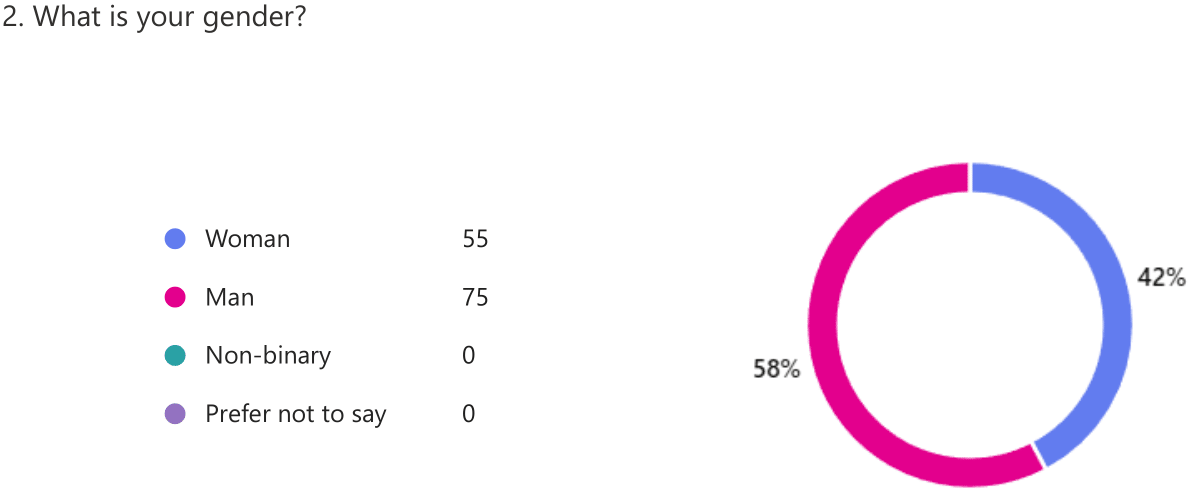
\includegraphics[width=\linewidth]{2}
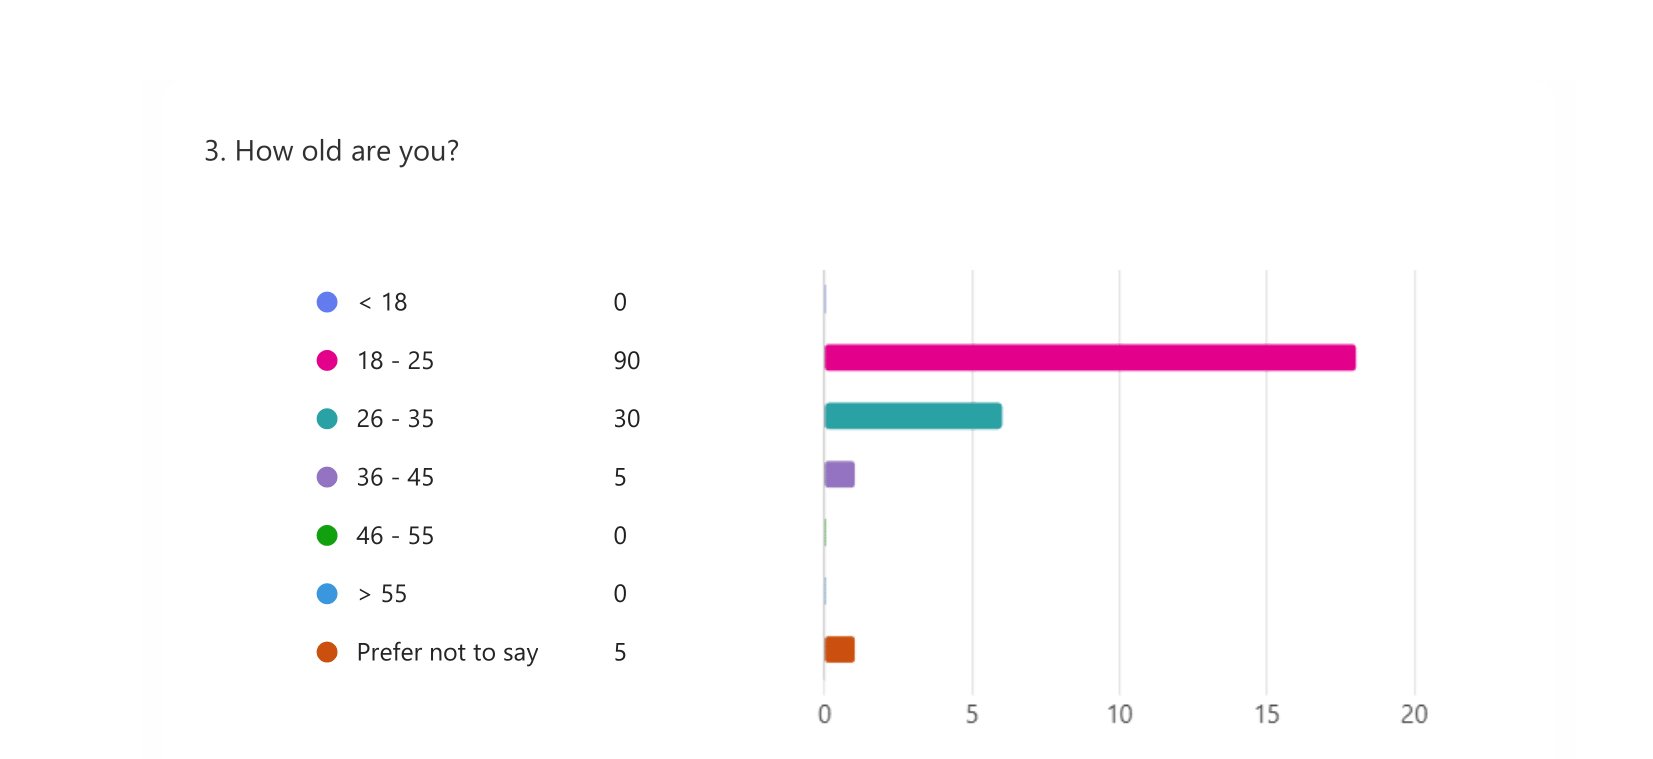
\includegraphics[width=\linewidth]{3}
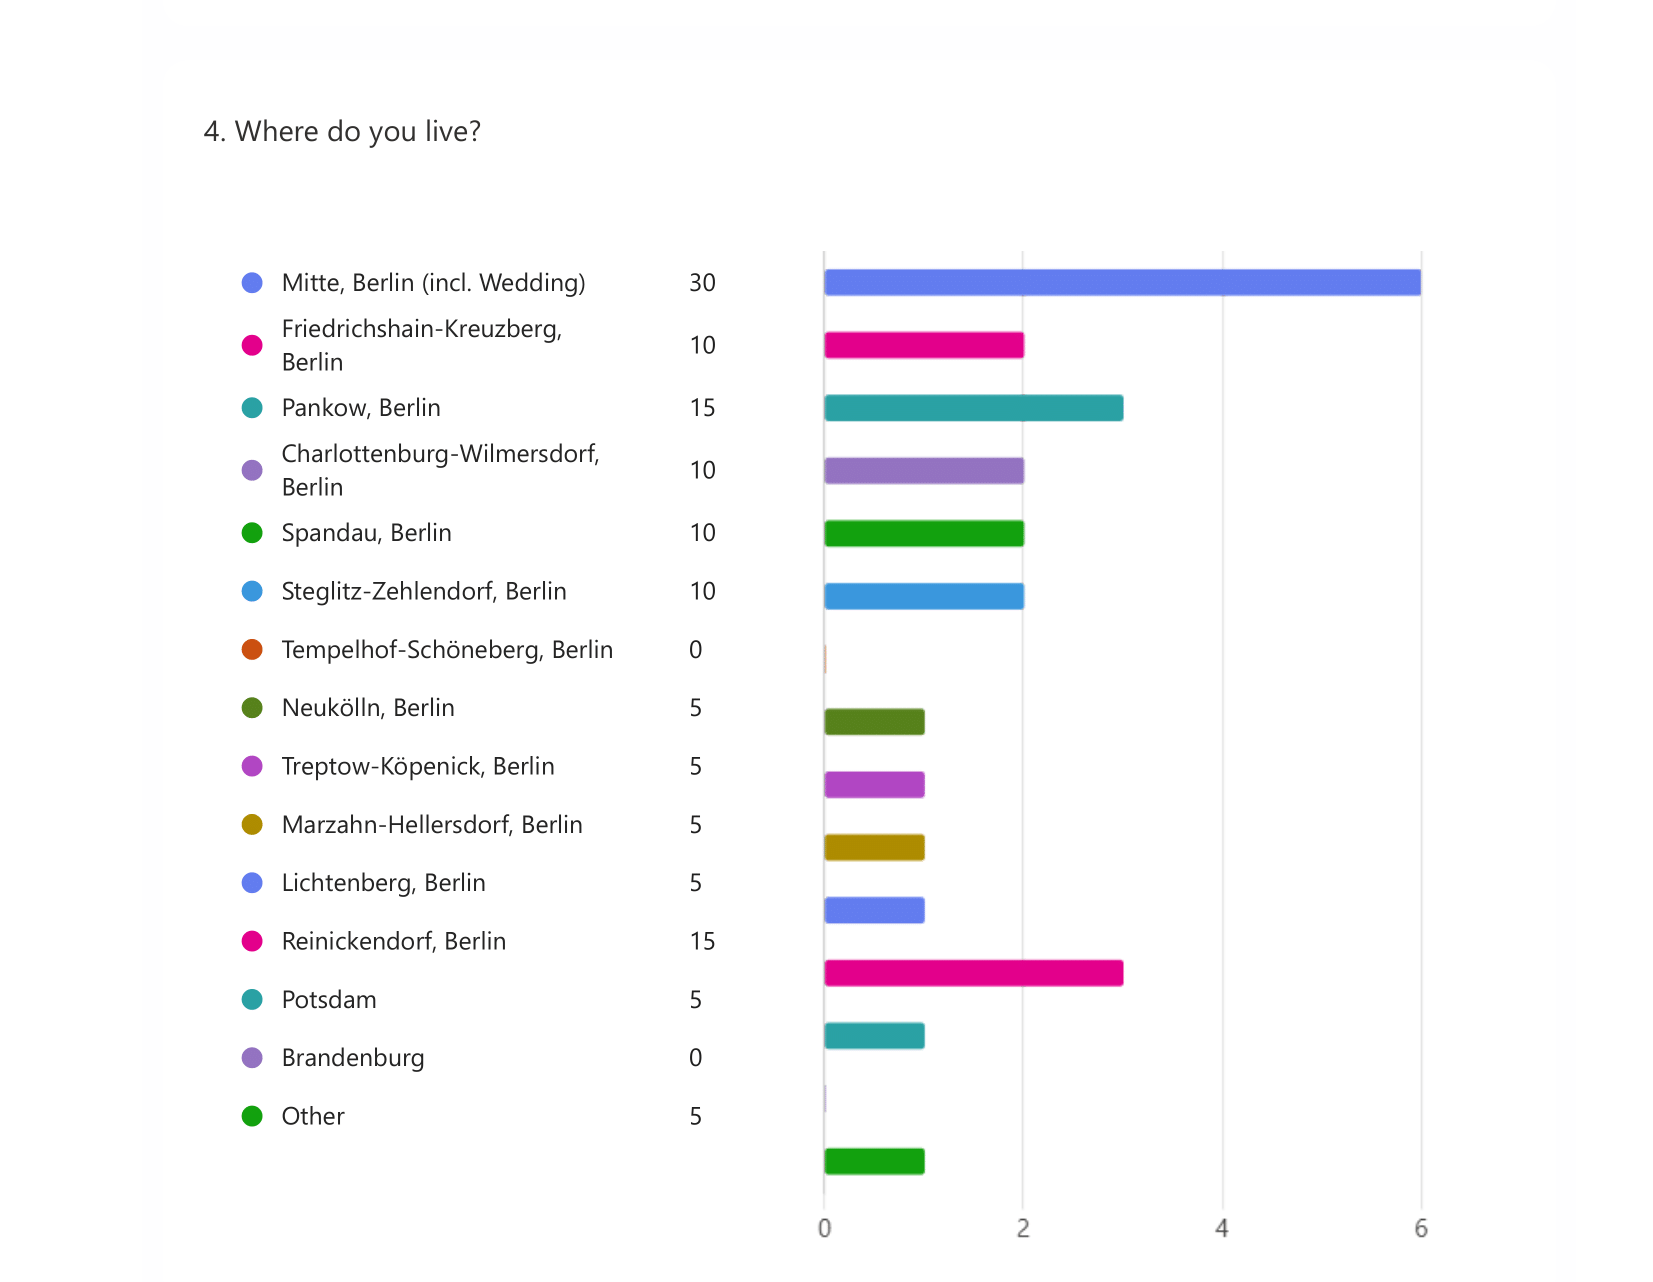
\includegraphics[width=\linewidth]{4}
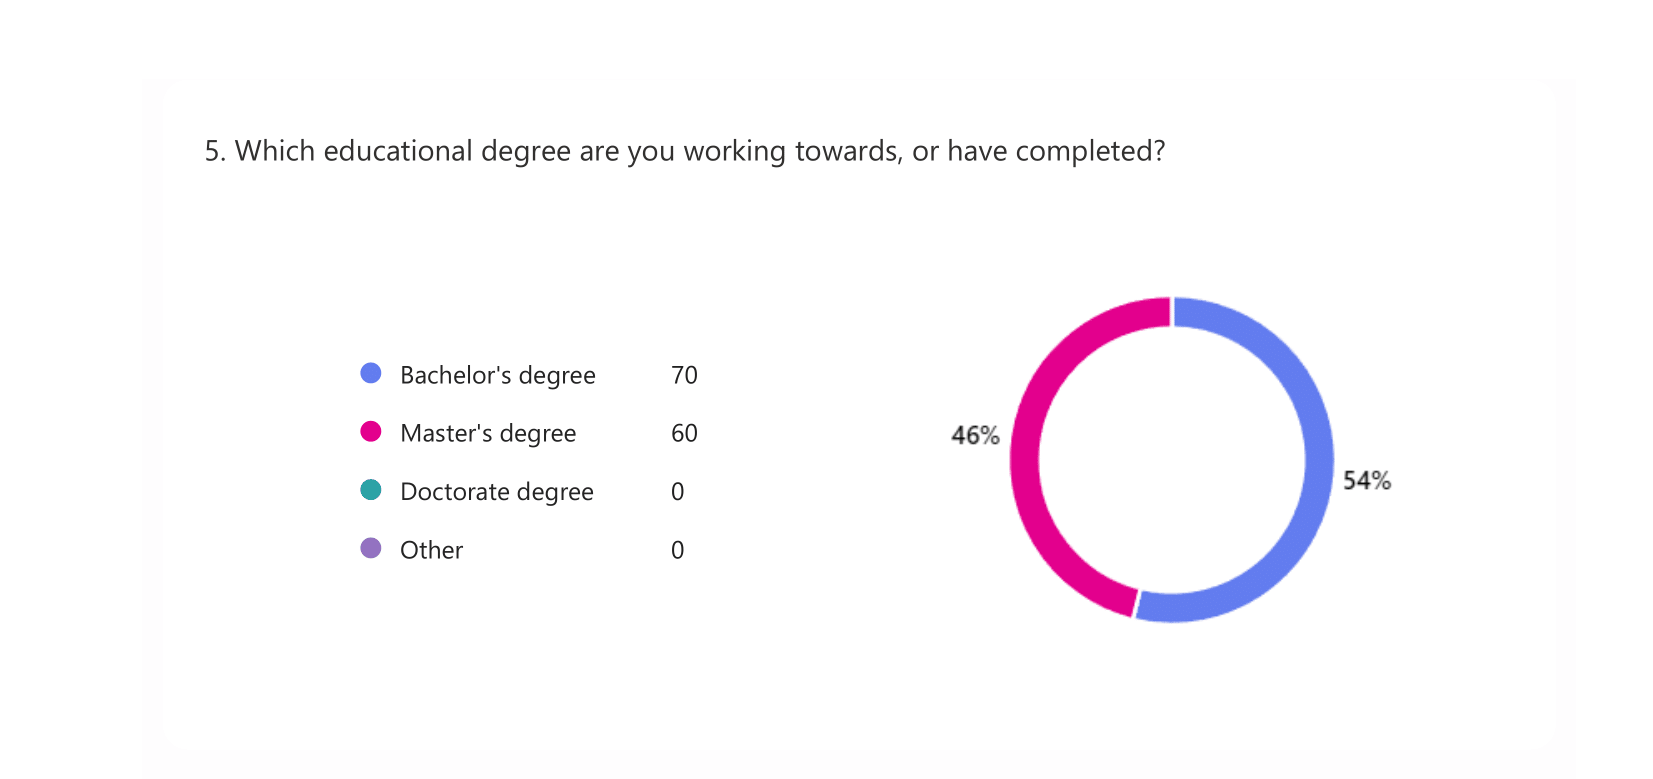
\includegraphics[width=\linewidth]{5}
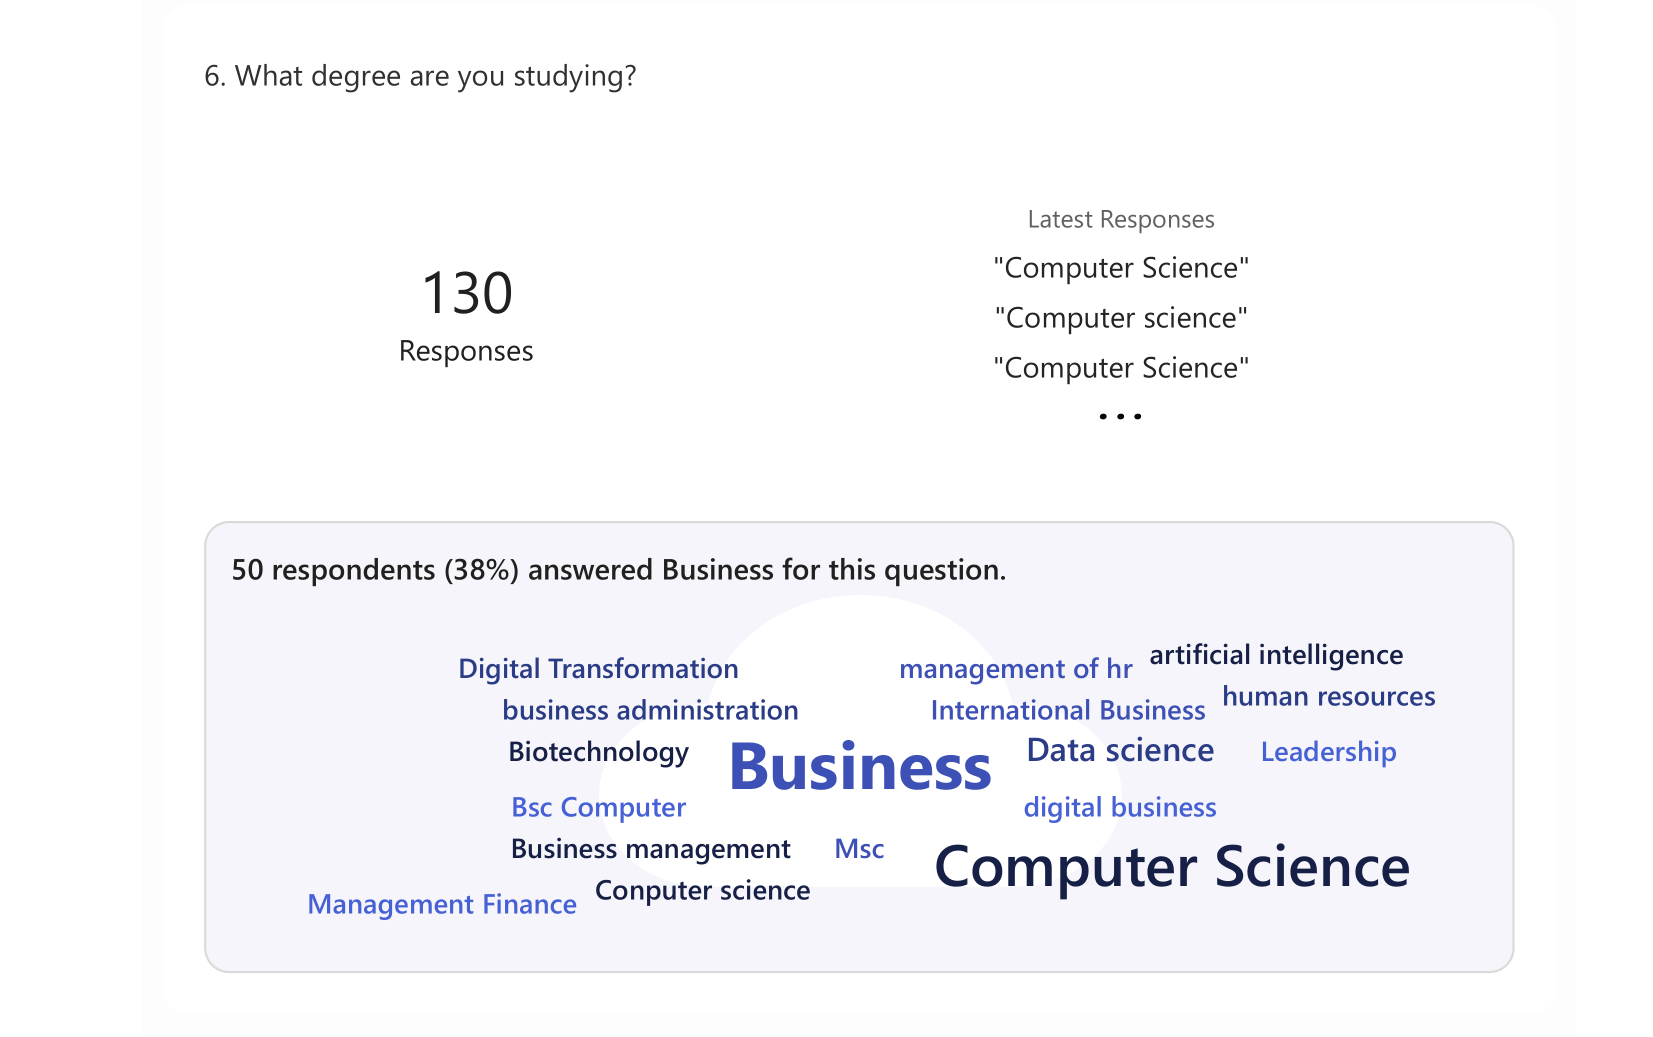
\includegraphics[width=\linewidth]{6}
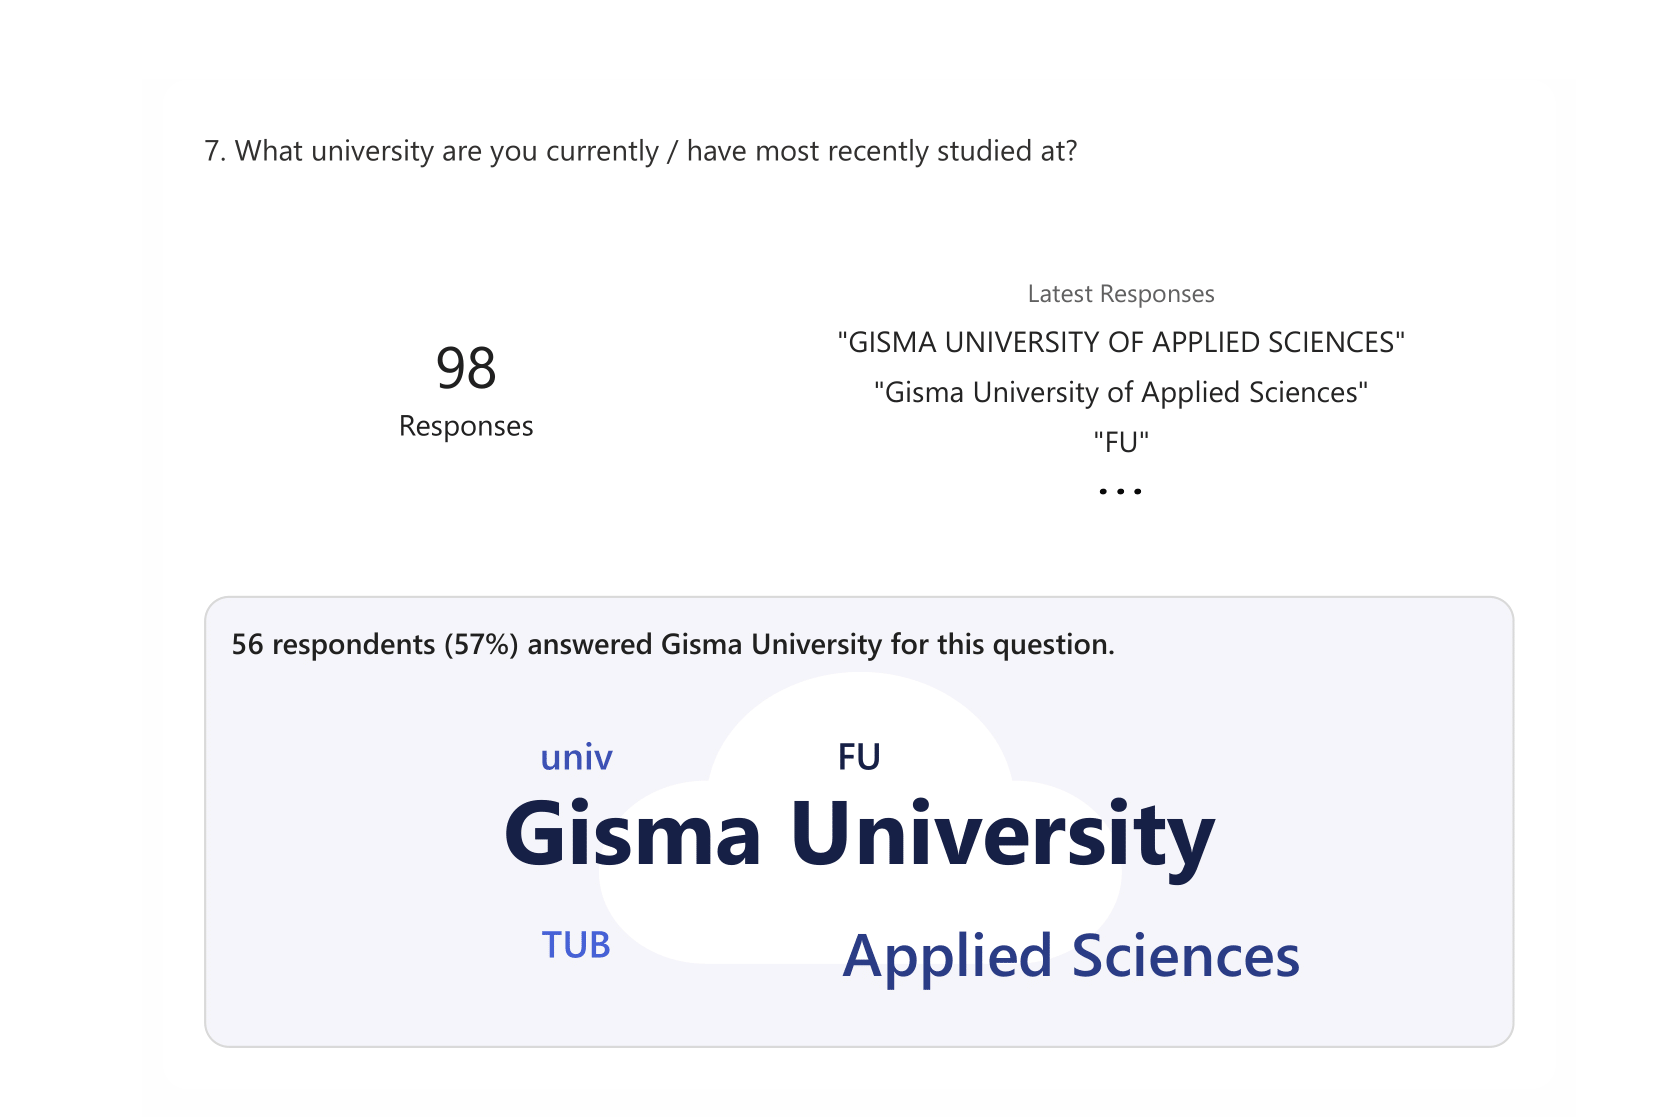
\includegraphics[width=\linewidth]{7}
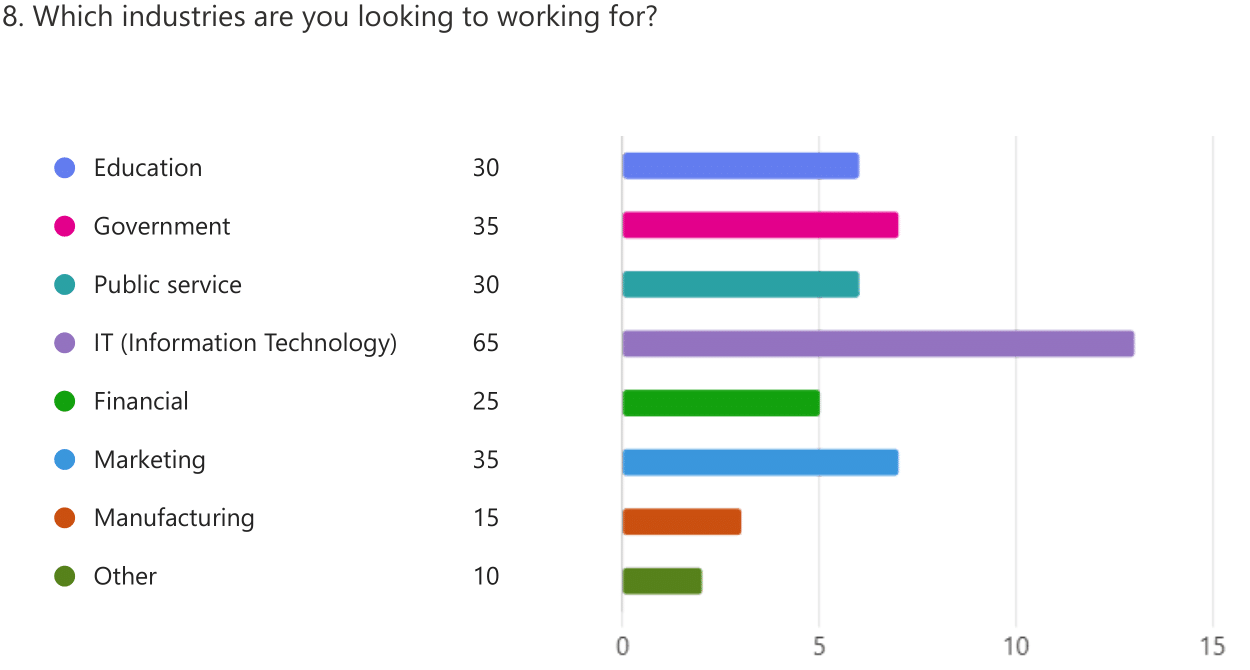
\includegraphics[width=\linewidth]{8}
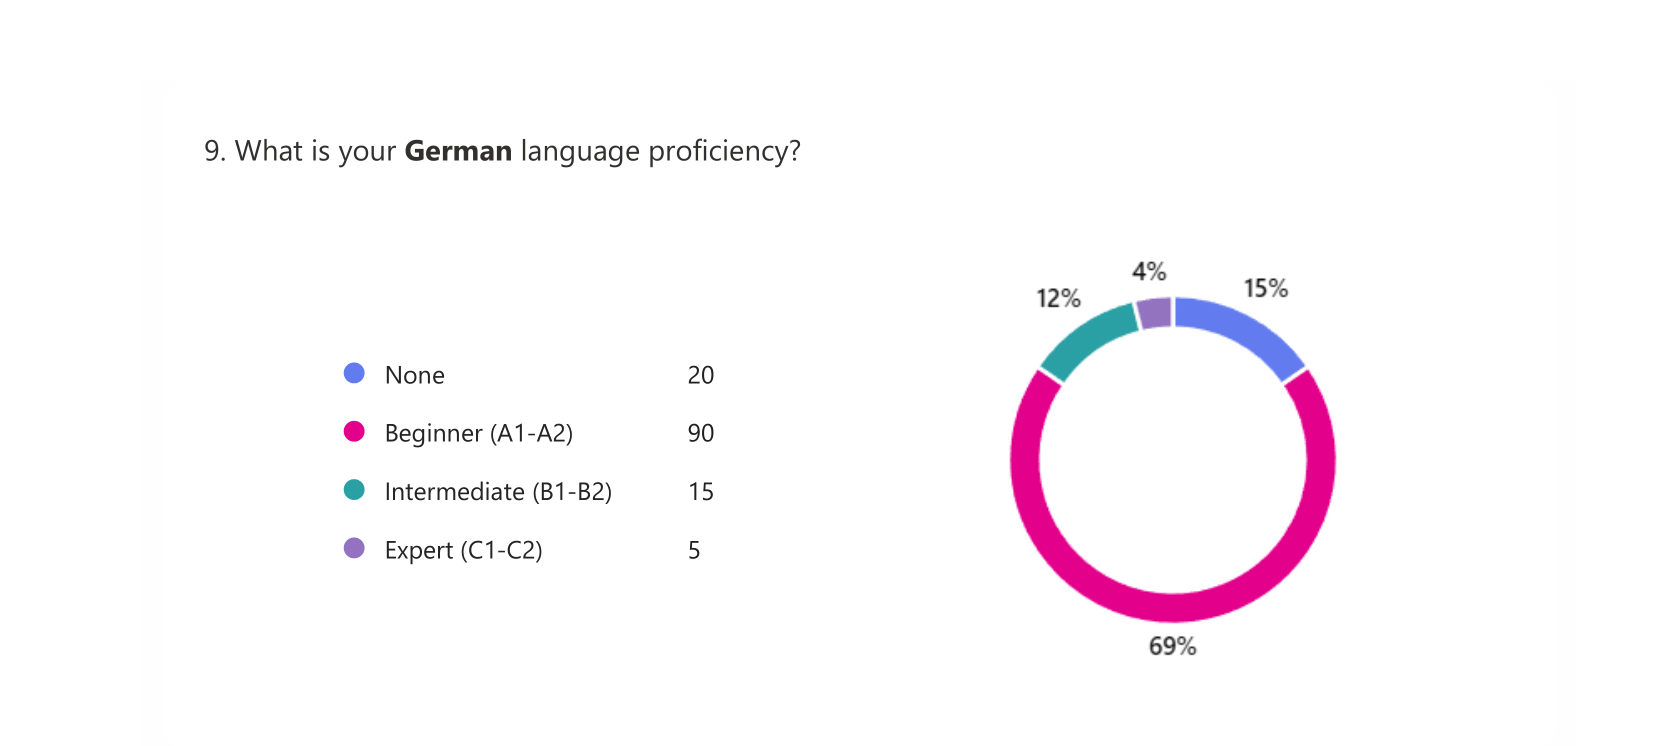
\includegraphics[width=11.09cm]{9}
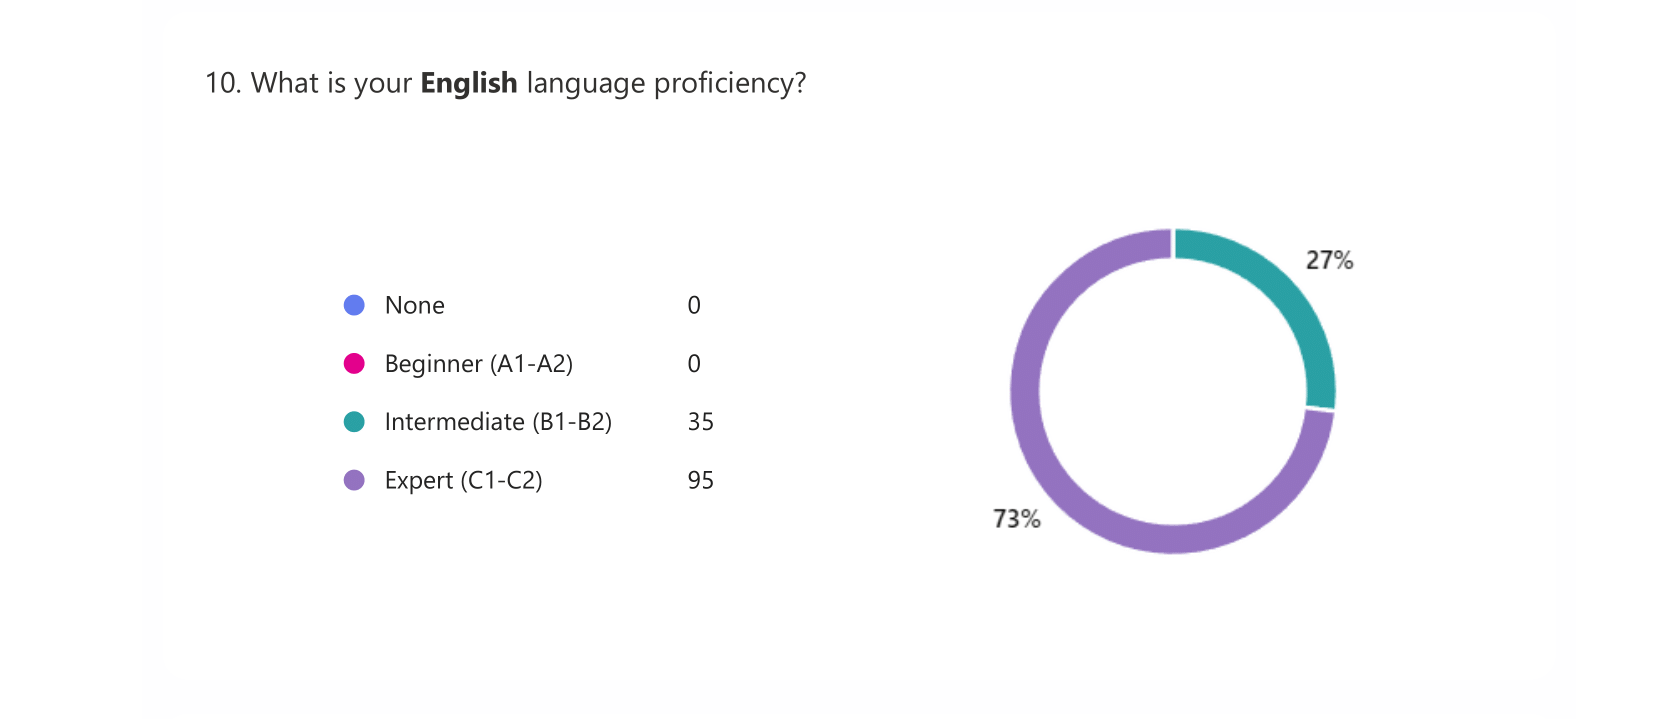
\includegraphics[width=11.18cm]{10}
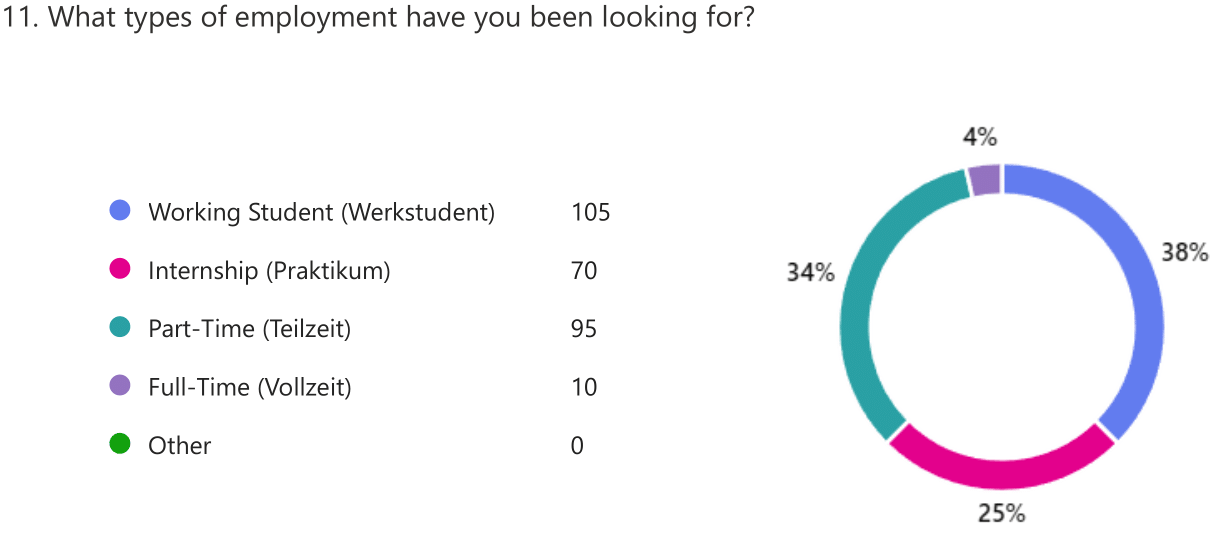
\includegraphics[width=11.79cm]{11}
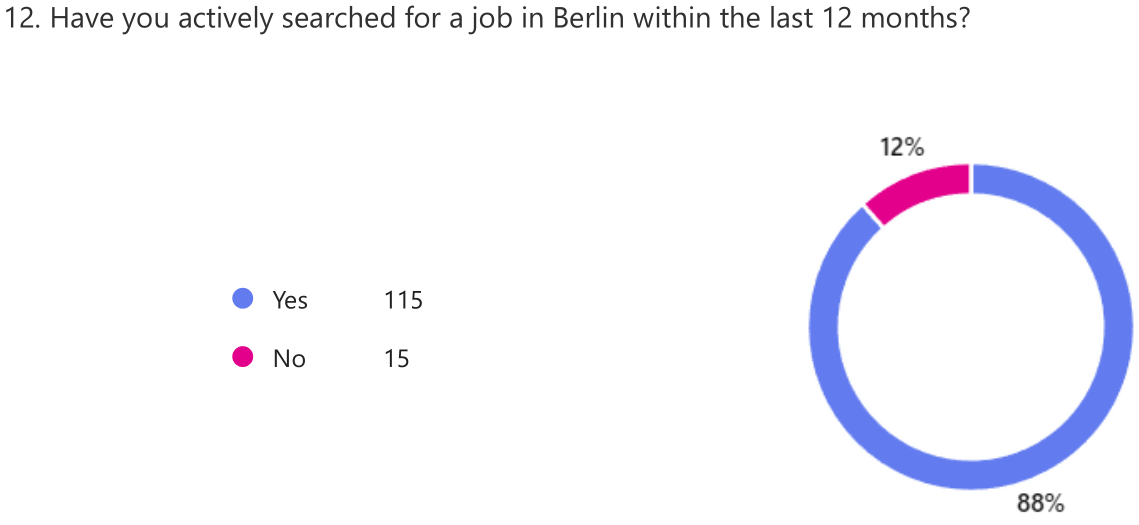
\includegraphics[width=11.11cm]{12}
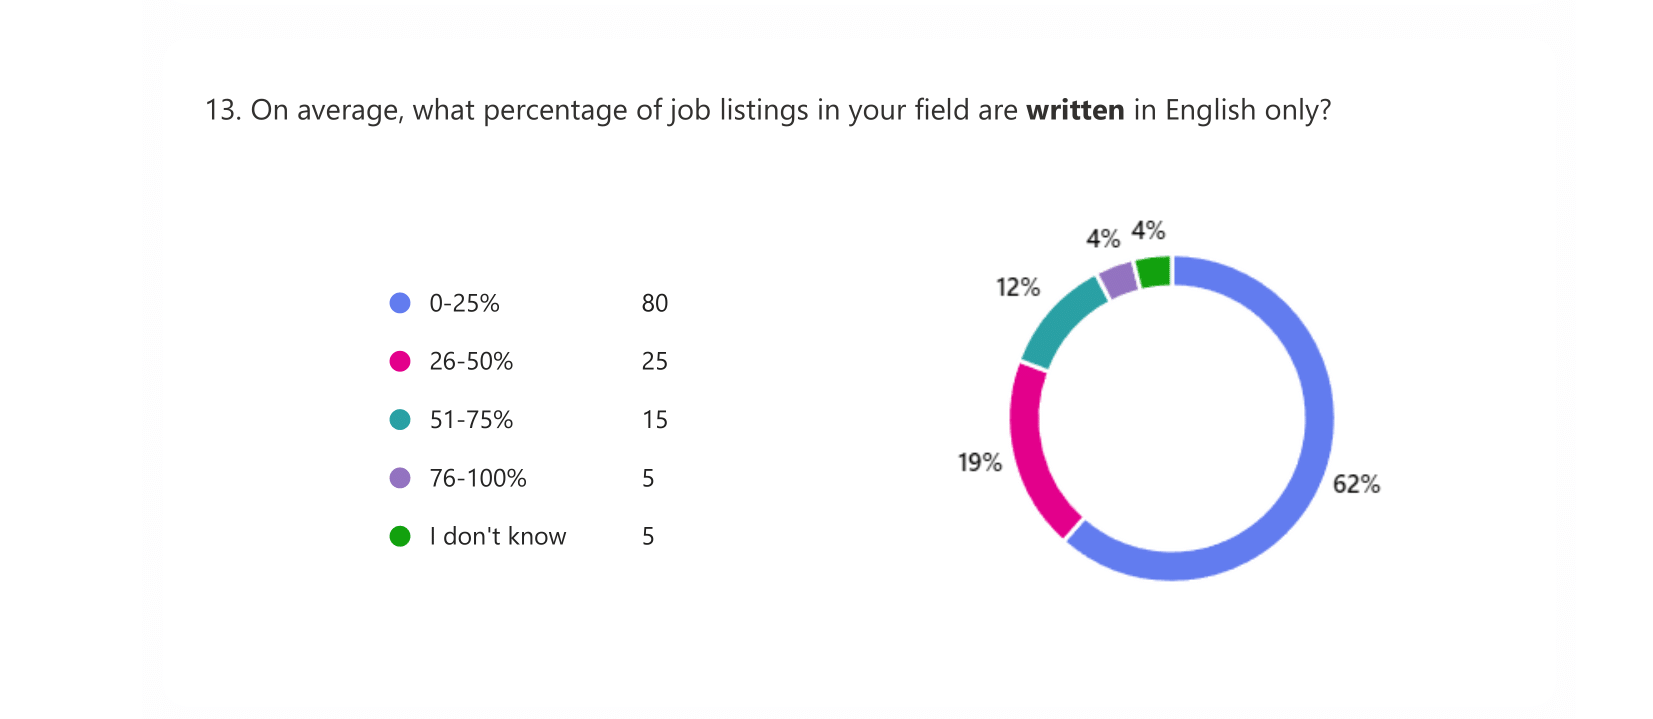
\includegraphics[width=11.54cm]{13}
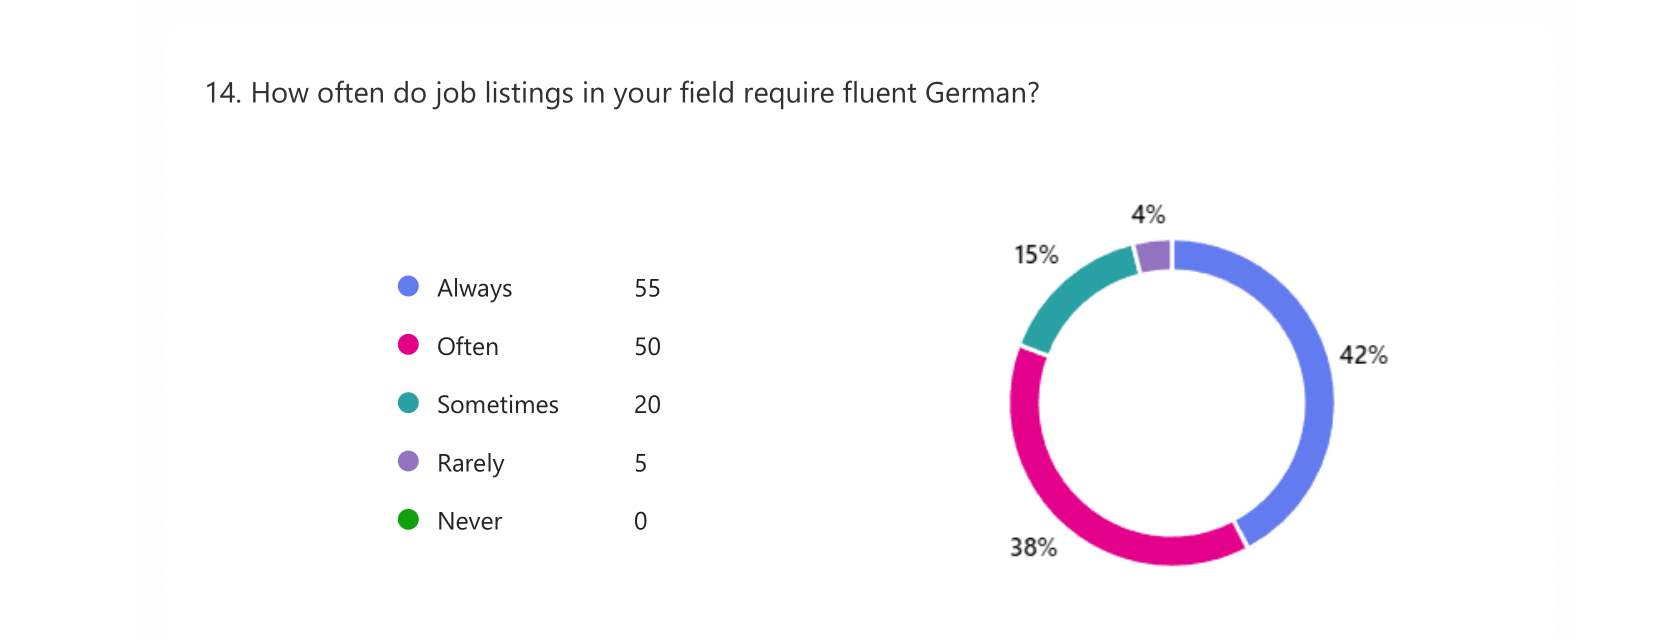
\includegraphics[width=11.48cm]{14}
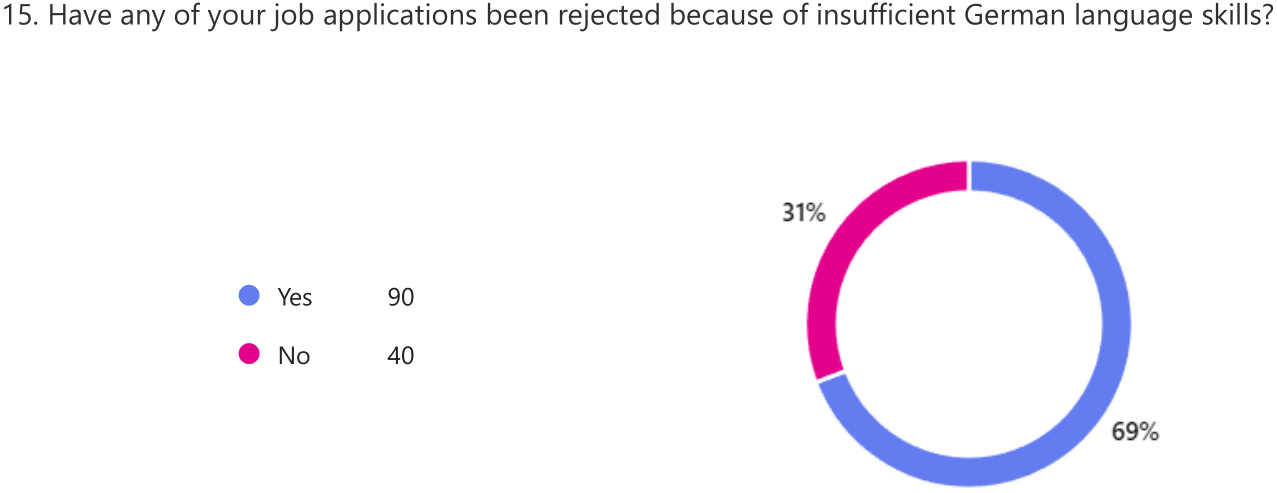
\includegraphics[width=12.41cm]{15}
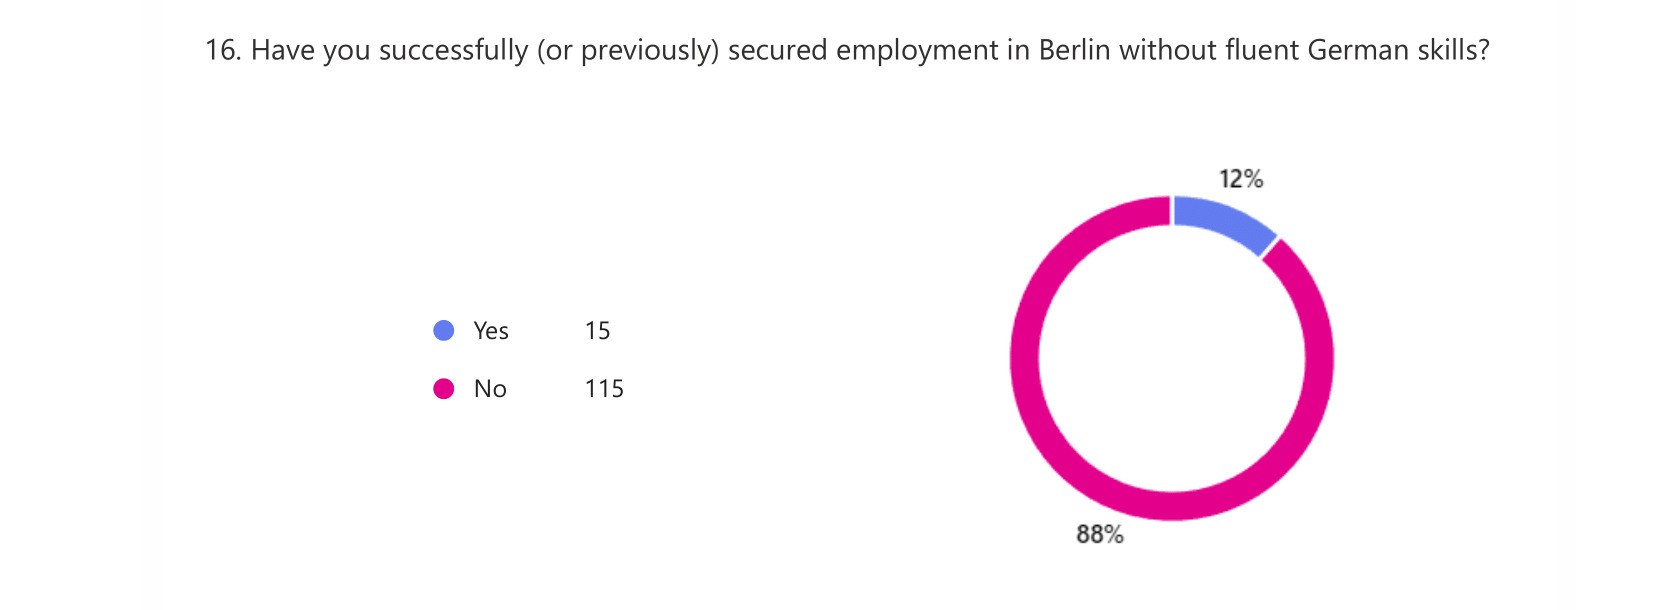
\includegraphics[width=12.52cm]{16}
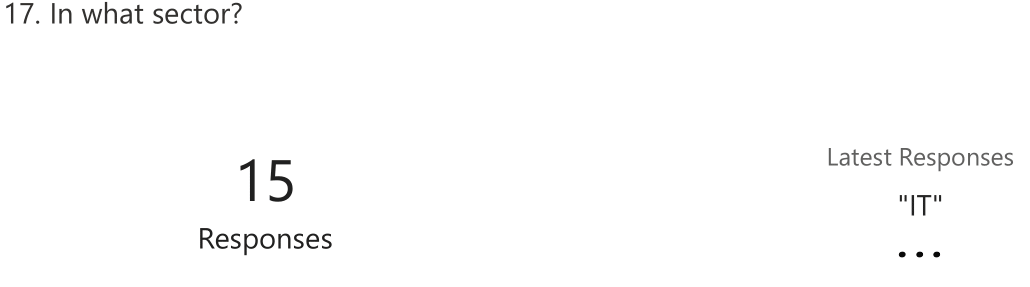
\includegraphics[width=10.43cm]{17}
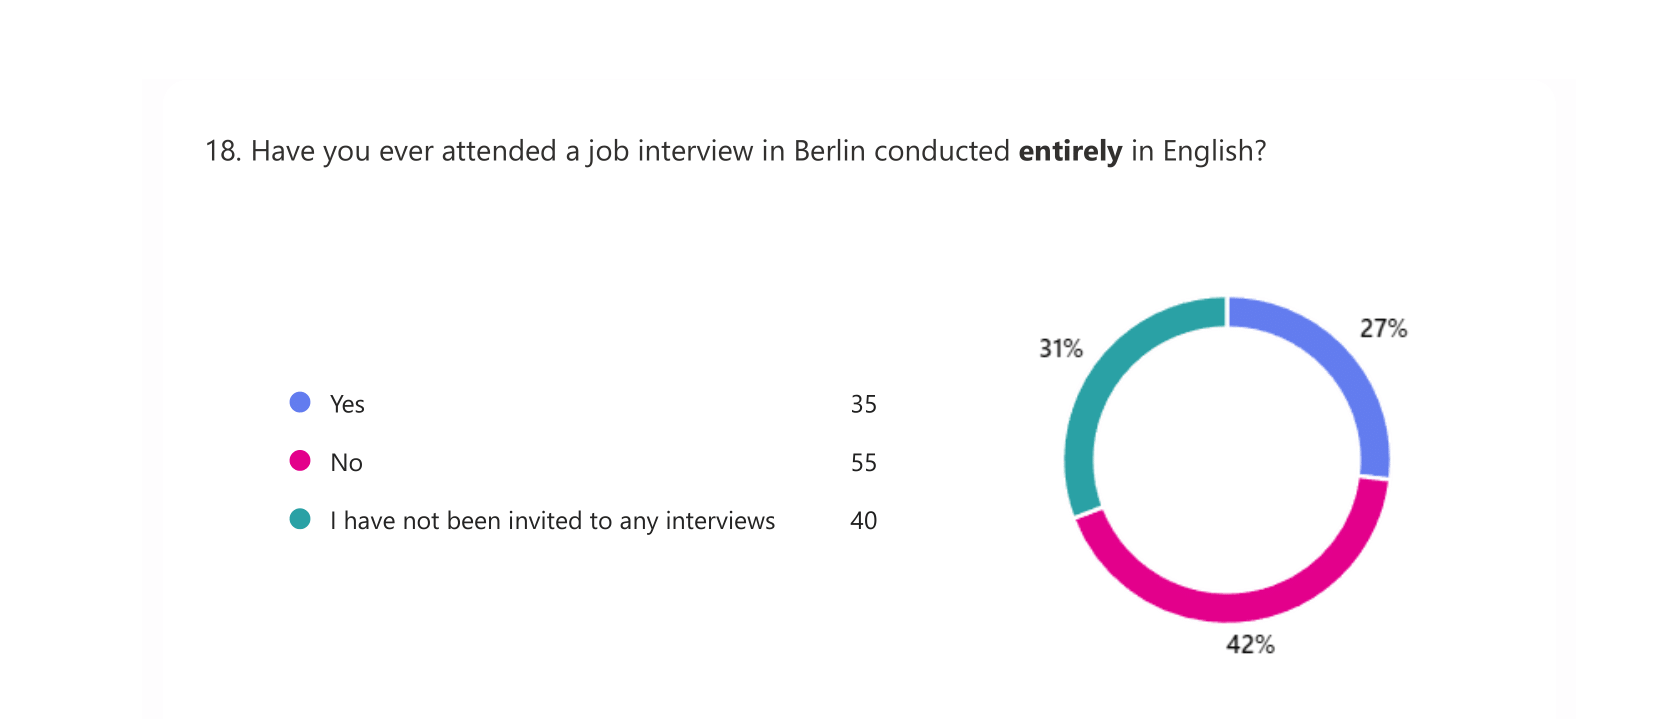
\includegraphics[width=11.8cm]{18}
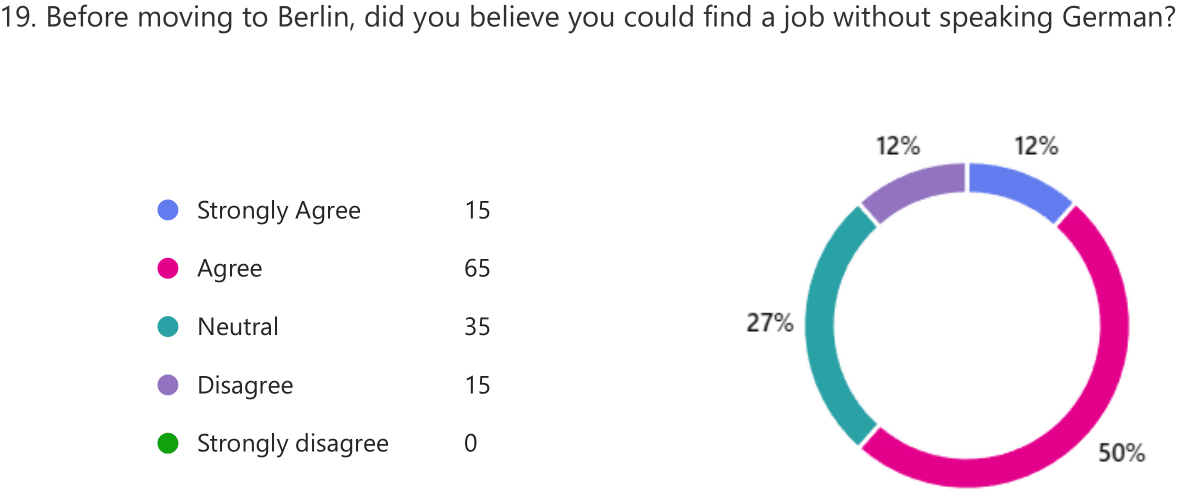
\includegraphics[width=11.62cm]{19}
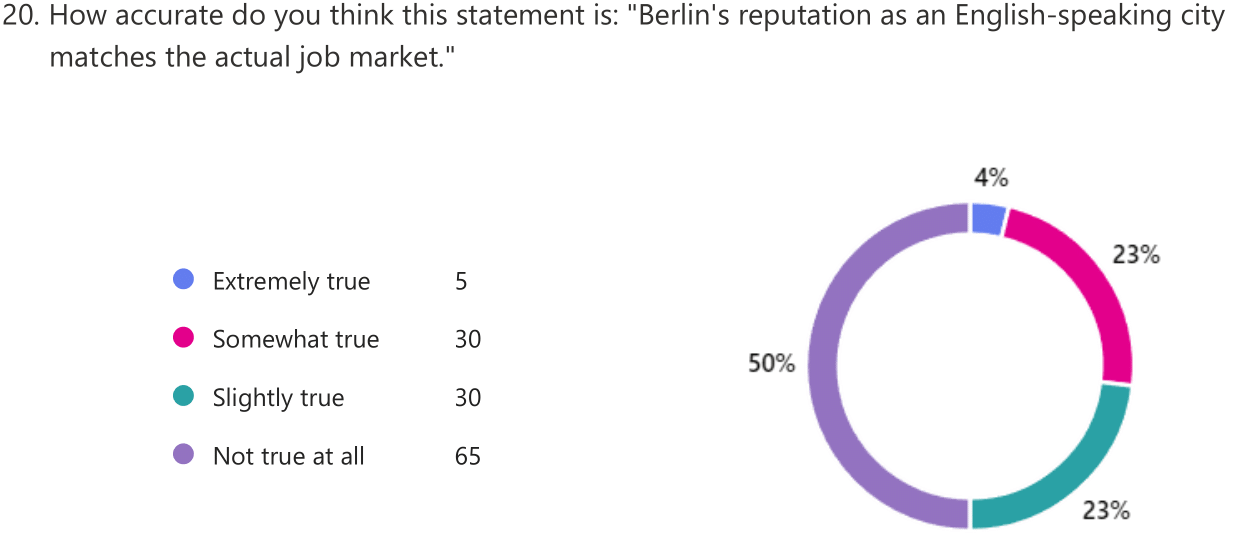
\includegraphics[width=12.73cm]{20}
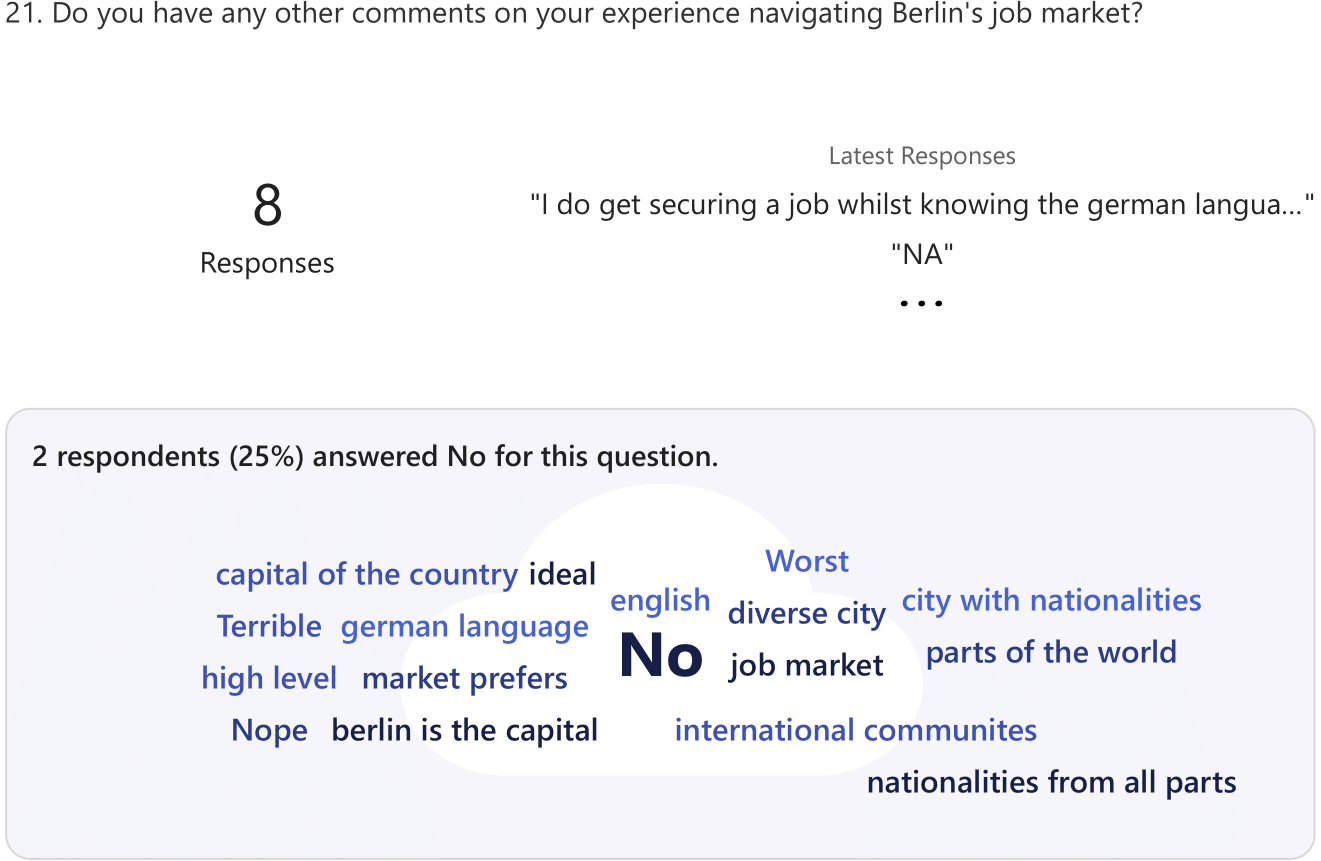
\includegraphics[width=12.94cm]{21}

\justifying
\clearpage